\section{Algorithms}\label{sec:algorithms}
This chapter describes how scalafmt formats Scala code.
We will see that scalafmt's design is inspired by ClangFormat and dartfmt.
However, we believe our design makes a valuable contribution in that it leverages functional programming principles to maximise code reuse and extensibility.

\subsection{Design}
Figure~\ref{fig:architecture} shows an architectural overview of scalafmt.
\begin{figure}
  \centering
  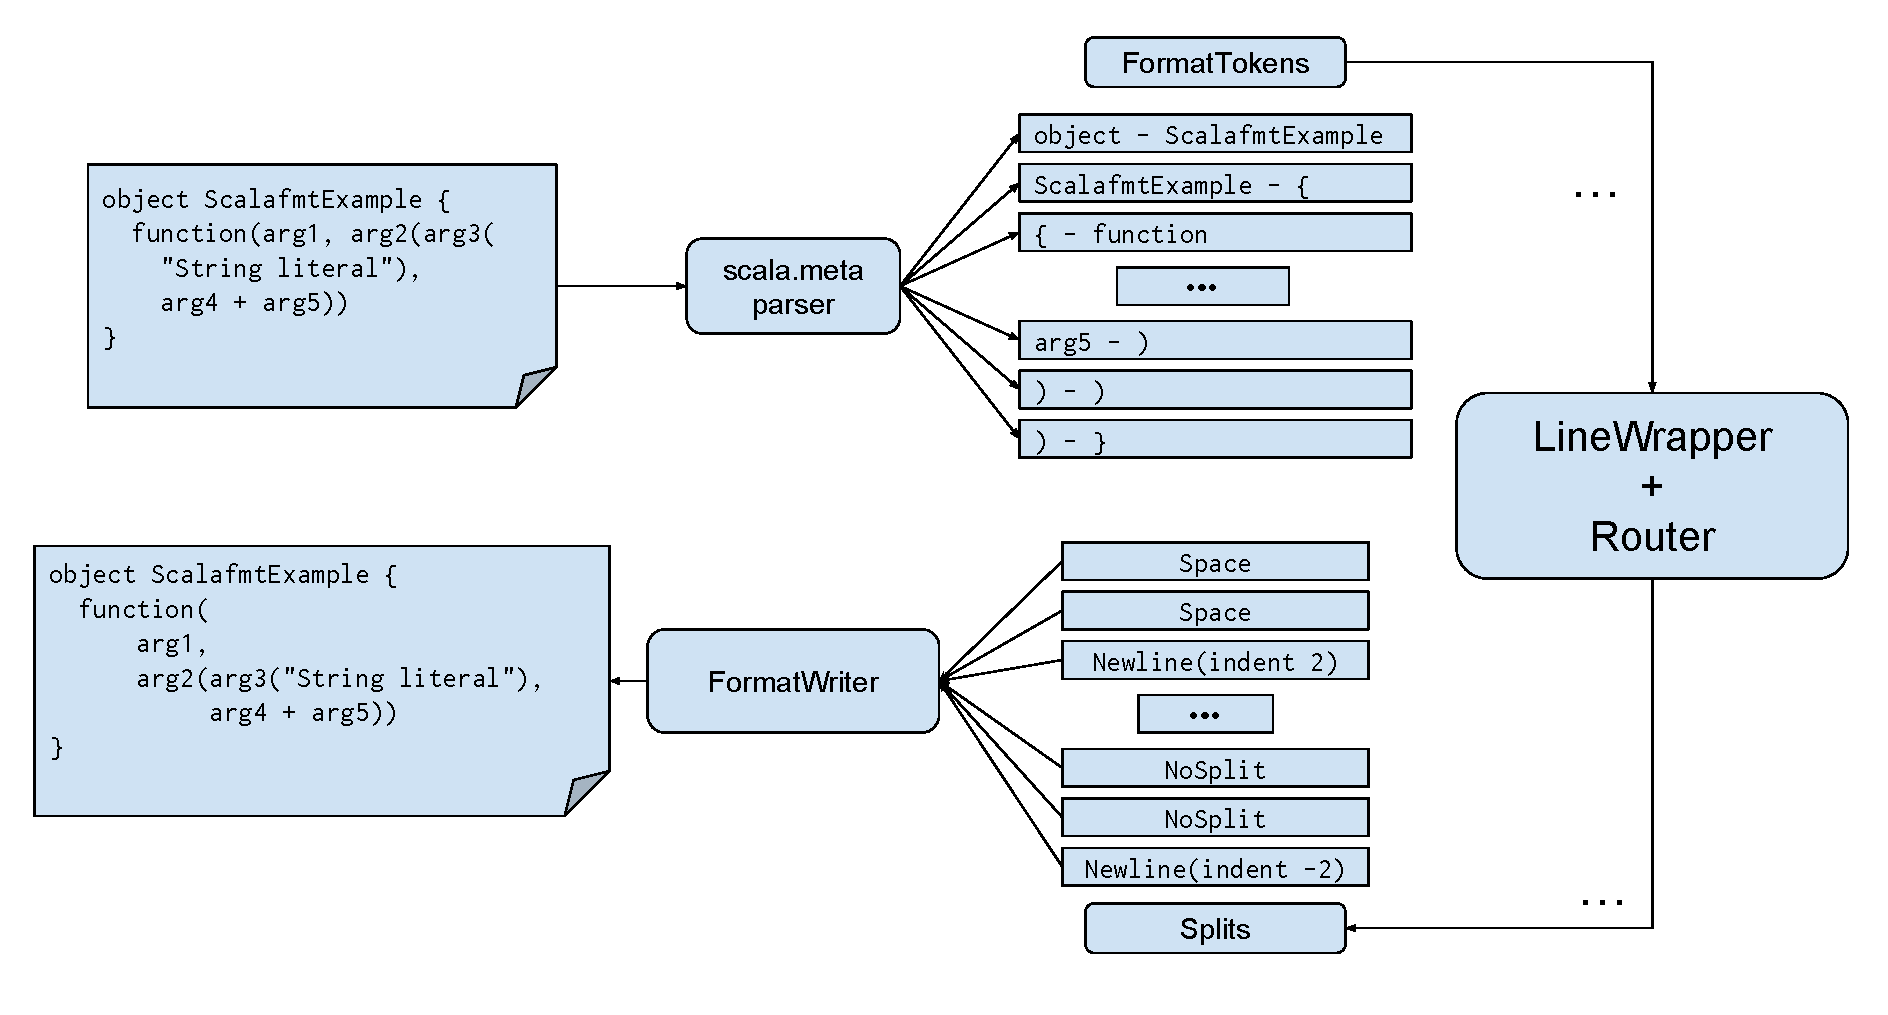
\includegraphics[width=\textwidth]{img/architechture.pdf}
  \caption{Scalafmt architecture}
  \label{fig:architecture}
\end{figure}
First, scalafmt parses a source file using scala.meta.
Next, we feed a sequence of \emph{FormatToken} data types into a \emph{LineWrapper}.
The LineWrapper uses a \emph{Router} to construct a weighted directed graph and run a best-first search to find an optimal formatting layout for the whole file.
Finally, the LineWrapper feeds a sequence of \emph{Split} data types into the \emph{FormatWriter}, which constructs a new reformatted source file.
In the next sections, we explain these data types and abstractions in detail.

\subsection{Data structures}
\subsubsection{FormatToken}
\subsubsection{Split}
\subsubsection{Indent}
\subsection{LineWrapper}
\subsubsection{Router}\label{sec:router}
\subsubsection{Policy}
\subsubsection{OptimalToken}
\subsubsection{State}
\subsection{Optimizations}
\subsubsection{dequeueOnNewStatements}
\subsubsection{recurseOnBlocks}
\subsubsection{escapeInPathologicalCases}
\subsubsection{escapeInPathologicalCases}
\subsubsection{pruneSlowStates}
\subsubsection{FormatWriter}
\begin{itemize}
  \item vertical alignment
  \item comment formatting
  \item stripMargin alignment
\end{itemize}
